5つの幅があり,各自の幅で各十回(毎回8分間)実験する,毎回の実験で,ランダムでロボットを2つグループを分ける.$T_{\rm sd}$と流量の平均値と分散を計測する
\begin{table}[!ht]
\setlength\tabcolsep{1pt}
\begin{center}
\begin{tabular}{|c|c|c|c|c|}
\hline
幅 & $T_{\rm sd}$(分) & $T_{\rm sd}$ & $Q$ & $Q$ \\
($m$)   &   平均値 & 標準偏差 & 平均値 & 標準偏差 \\
\hline
0.43 & 8.0 & 0 & 0.436 & 0.145 \\
\hline
0.495 & 6.572 & 137.346 & 3.216 & 2.814 \\
\hline
0.56 & 4.63 & 133.561 & 5.248 & 3.394 \\
\hline
0.625 & 4.568 & 106.722 & 3.29 & 2.774 \\
\hline
0.69 & 4.556 & 139.082 & 5.413 & 3.501 \\
\hline
\end{tabular}
\end{center}
\caption{
幅により$T_{\rm sd}$と流量の値
}
\end{table}
\vspace{-6mm}
\begin{figure}[!ht]
    \centering
    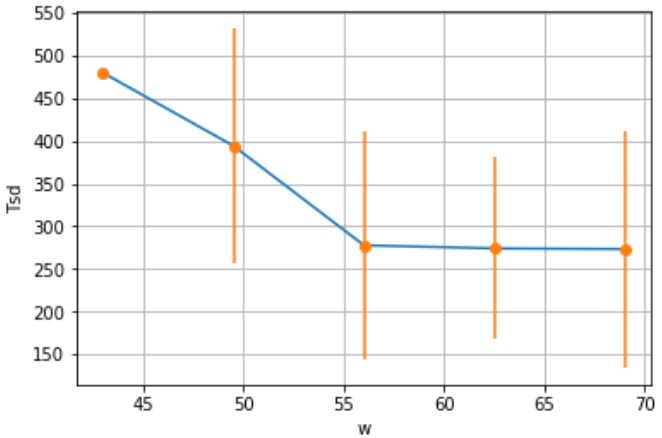
\includegraphics[width=0.8\linewidth]{diagram3.jpg}
    \caption{$T_{\rm sd}$とコース幅の関係}
\end{figure}
\vspace{-6mm}
\begin{figure}[!ht]
    \centering
    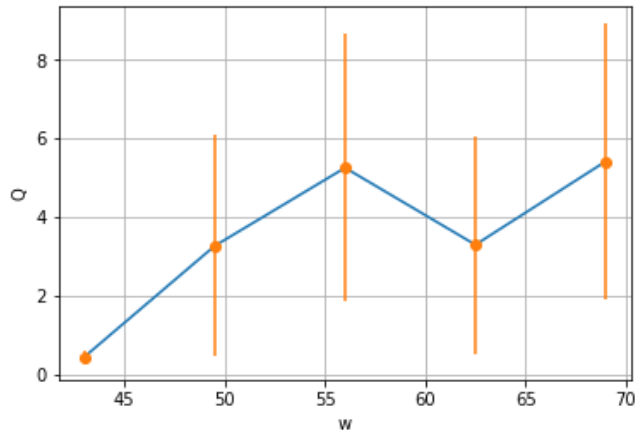
\includegraphics[width=0.8\linewidth]{diagram4.jpg}
    \caption{$Q$とコース幅の関係}
\end{figure}

図$7$は幅の拡大に従って,平均$T_{\rm sd}$の変化曲線である.図$8$が幅の拡大に従って,平均流量($Q$)の変化曲線である.幅が狭すぎる(43$cm$)と,長時間の渋滞が発生したことを観測した,ロボット同士が互いに引っかかって,方向転換もできなくて,one direction flow の状態も出なかった.大渋滞ので,流量もほとんどない.49.5$cm$の場合,渋滞も起こったので,one direction flow 状態になる時間($T_{\rm sd}$)も長かった,ロボットがギリギリ方向転換できて,流量も多少増えてきた.56$cm$から渋滞がほとんどなくて,ロボットの方向転換もしやすくなって,$T_{\rm sd}$が減少して,幅がもっと広まっても,あんまり変わらないようになった.56$cm$まで平均流量が増えて,$62.5cm$の場合,平均流量が多少減少したと観測した.

